\documentclass[12pt]{article}

%Begin----------------------------------------------------------------------------------------------------------------------------------------
%---------------------------------------------------------------------------------------------------------------------------------------------
%Package import and Config of Packages
%\usepackage[utf8]{inputenc}%\usepackage{tikz}#
\usepackage{lmodern}
\usepackage{setspace}
\usepackage{lastpage}
\usepackage{pgfplots} % Fuer Plots
\usepackage{pgfplotstable}
\usepackage{pgfkeys} 
\usepackage{filecontents}
\pgfplotsset{compat = newest}
\usepackage{tikz} % Generell gutes Packet
\usepackage{csvsimple} % Zum CSV auslesen
\usepackage{fancyhdr}
\usepackage{tcolorbox}
\usepackage{lipsum}
\usepackage{circuitikz}
\usepackage[T1]{fontenc}
\usepackage[scaled]{helvet}
\renewcommand{\familydefault}{\sfdefault}

\usepackage[ngerman]{babel}
\usepackage{datetime}
\newdateformat{myformat}{\THEDAY{ten }\monthname[\THEMONTH], \THEYEAR}

\usepackage[LGRgreek]{mathastext}
\usepackage{enumerate}
\usepackage{cancel}
\usepackage{subfig}
\usepackage{pdfpages}
\usepackage{subfiles}
\usepackage{titlesec}
\usepackage[pdfborder={0 0 0}]{hyperref}
\usepackage{pdfpages}
\usepackage{verbatim}
\usepackage{geometry}
\geometry{left=20mm, right=20mm, bottom=20mm}

\usepackage{graphicx}
\graphicspath{{../Bilder/}{Bilder/}}


%End------------------------------------------------------------------------------------------------------------------------------------------
%---------------------------------------------------------------------------------------------------------------------------------------------
%Package import and Config of Packages

%Begin----------------------------------------------------------------------------------------------------------------------------------------
%---------------------------------------------------------------------------------------------------------------------------------------------
%List Configuration for Coding
\usepackage{listings} % Generell Code-Boxen
\usepackage{xcolor} % Fuer extra Farben mit color{}

\colorlet{punct}{red!60!black}
\definecolor{background}{HTML}{EEEEEE}
\definecolor{delim}{RGB}{20,105,176}
\colorlet{numb}{magenta!60!black}

\definecolor{mGreen}{rgb}{0,0.6,0}
\definecolor{mGray}{rgb}{0.5,0.5,0.5}
\definecolor{mPurple}{rgb}{0.58,0,0.82}
\definecolor{backgroundColour}{rgb}{255,255,255}

\lstdefinestyle{CStyle}
{
    backgroundcolor=\color{backgroundColour},   
    belowcaptionskip=1\baselineskip,
    breaklines=true,
    xleftmargin=\parindent,
    language=C,
    frame = single,
    showstringspaces=false,
    basicstyle=\footnotesize\ttfamily,
    keywordstyle=\bfseries\color{magenta},
    commentstyle=\color{mGreen},
    identifierstyle=\color{blue},
    stringstyle=\color{orange},
} 

%End------------------------------------------------------------------------------------------------------------------------------------------
%---------------------------------------------------------------------------------------------------------------------------------------------
%List Configuration for Coding


%Begin----------------------------------------------------------------------------------------------------------------------------------------
%---------------------------------------------------------------------------------------------------------------------------------------------
%More Subsections Configuration
\titleclass{\subsubsubsection}{straight}[\subsection]
\newcounter{subsubsubsection}[subsubsection]
\renewcommand\thesubsubsubsection{\thesubsubsection.\arabic{subsubsubsection}}
\renewcommand\theparagraph{\thesubsubsubsection.\arabic{paragraph}} % optional; useful if paragraphs are to be numbered
\titleformat{\subsubsubsection}
  {\normalfont\normalsize\bfseries}{\thesubsubsubsection}{1em}{}
\titlespacing*{\subsubsubsection}
{0pt}{3.25ex plus 1ex minus .2ex}{1.5ex plus .2ex}


\titleclass{\subsubsubsubsection}{straight}[\subsection]
\newcounter{subsubsubsubsection}[subsubsubsection]
\renewcommand\thesubsubsubsubsection{\thesubsubsubsection.\arabic{subsubsubsubsection}}
\titleformat{\subsubsubsubsection}
  {\normalfont\normalsize\bfseries}{\thesubsubsubsubsection}{1em}{}
\titlespacing*{\subsubsubsubsection}
{0pt}{3.25ex plus 1ex minus .2ex}{1.5ex plus .2ex}

\makeatletter
\renewcommand\paragraph{\@startsection{paragraph}{5}{\z@}%
  {3.25ex \@plus1ex \@minus.2ex}%
  {-1em}%
  {\normalfont\normalsize\bfseries}}
\renewcommand\subparagraph{\@startsection{subparagraph}{6}{\parindent}%
  {3.25ex \@plus1ex \@minus .2ex}%
  {-1em}%
  {\normalfont\normalsize\bfseries}}
\def\toclevel@subsubsubsection{4}
\def\toclevel@paragraph{5}
\def\toclevel@paragraph{6}
\def\l@subsubsubsection{\@dottedtocline{4}{7em}{4em}}
\def\l@subsubsubsubsection{\@dottedtocline{5}{8em}{5em}}
\def\l@paragraph{\@dottedtocline{5}{10em}{5em}}
\def\l@subparagraph{\@dottedtocline{6}{14em}{6em}}
\makeatother

\setcounter{secnumdepth}{5}
\setcounter{tocdepth}{5}

%End------------------------------------------------------------------------------------------------------------------------------------------
%---------------------------------------------------------------------------------------------------------------------------------------------
%More Subsections Configuration


\pagestyle{fancy}
\fancyhf{}


%Begin----------------------------------------------------------------------------------------------------------------------------------------
%---------------------------------------------------------------------------------------------------------------------------------------------
%TitelSeite
\title{FSST: QSort}
\author{Fabio~Plunser \\ Betreuer: Roland~Lezuo}
\date{\today}
\rhead{\hspace{5px}
\includegraphics[scale=0.09]{Bilder/logo.png}}
\lhead{FSST: QSort}
\rfoot{Page~\thepage ~of~\pageref{LastPage}}
\lfoot{PlunserFabio}
\renewcommand{\headrulewidth}{1pt}
\renewcommand{\footrulewidth}{1pt}



\begin{document}
\pagenumbering{gobble}

\begin{titlepage}
	\maketitle
\end{titlepage}

%End------------------------------------------------------------------------------------------------------------------------------------------
%---------------------------------------------------------------------------------------------------------------------------------------------
%TitelSeite

%Begin----------------------------------------------------------------------------------------------------------------------------------------
%---------------------------------------------------------------------------------------------------------------------------------------------
%Inhaltsverzeichnis
\pagebreak
\thispagestyle{empty}
\renewcommand\contentsname{Inhaltsverzeichnis}
\tableofcontents	
\pagenumbering{gobble}

%End------------------------------------------------------------------------------------------------------------------------------------------
%---------------------------------------------------------------------------------------------------------------------------------------------
%Inhaltsverzeichnis

%Begin----------------------------------------------------------------------------------------------------------------------------------------
%---------------------------------------------------------------------------------------------------------------------------------------------
%Abbildungsverzeichnis
% \pagebreak
\thispagestyle{empty}
\renewcommand\listfigurename{Abbildungsverzeichnis}
\listoffigures
%End------------------------------------------------------------------------------------------------------------------------------------------
%---------------------------------------------------------------------------------------------------------------------------------------------
%Abbildungsverzeichnis


%Begin----------------------------------------------------------------------------------------------------------------------------------------
%---------------------------------------------------------------------------------------------------------------------------------------------
%Codeverzeichnis
% \renewcommand\lstlistlistingname{Codeverzeichnis}
% \lstlistoflistings
\pagebreak
\pagenumbering{arabic}

%End------------------------------------------------------------------------------------------------------------------------------------------
%---------------------------------------------------------------------------------------------------------------------------------------------
%Codeverzeichnis



%Begin----------------------------------------------------------------------------------------------------------------------------------------
%---------------------------------------------------------------------------------------------------------------------------------------------
%Main
% \newpage
\section{Aufgabenstellung}
    \begin{lstlisting}[language=Python, style=Stylepython, caption=Angabge, captionpos=b, label=Angabge]
# deciphers to "Schoene Crypto Welt" with IV=BBBBBBBBBBBBBBBB and key=BBBBBBBBBBBBBBBB aes128-cbc
cyphertext = "AAE365272C81078AB6116B361831D0F6A5D3C8587E946B530B7957543107F15E"
bc = binascii.unhexlify(cyphertext)
data = b'D' + bytes([len(bc)]) + binascii.unhexlify(cyphertext) + b'X'  
\end{lstlisting}
    
\noindent  Der cyphertext soll entschlüsselt \anfuehrung{Schöne Crypto Welt} bedeuten. 
Um dies zu überprüfen kann \href{OpenSSL}{https://www.openssl.org/} verwendet werden.\\

\noindent Schreiben Sie ein Programm das unter Verwendnung von openssl obige Aussage überprüft, 
verbessen Sie ihr Program in dem Sinne dass sie key/iv/plaintexte/ciphertexte als Argumente/Dateien/Usereingaben verarbeiten.

\subsection*{Hinweise}
\begin{itemize}
    \item Sie benötigen die openssl Biblotheksheader, unter Ubuntu 20.04 können Sie diese installieren via:
    \begin{lstlisting}[language=Python, style=Stylepython, caption=Angabge, captionpos=b, label=Angabge]
$ sudo apt install libssl-dev
    \end{lstlisting}
    
    \item em Linker muss mitgeteilt werden dass sie in Ihrem Programm Funktionen verwenden die in einer externen Bibliothek bereit liegen, verwenden 
    sie dazu das flag -l (klein-L) und den Namen der Bibliothek OHNE das führende lib. 
    openssl besteht aus mehreren Bibliotheken, die für AES notwendingen Funktionen befinden sich in libcrypto.
    \begin{lstlisting}[language=Python, style=Stylepython, caption=Angabge, captionpos=b, label=Angabge]
$ gcc my_code.c -lbibliothek -o my_executable
    \end{lstlisting}
    Sie können sich die gelinkten Bibliotheken dann via ldd Kommando ansehen
    \begin{lstlisting}[language=Python, style=Stylepython, caption=Angabge, captionpos=b, label=Angabge]
$ ldd my_executable
    \end{lstlisting}
\end{itemize}

\newpage
\section{Angabe}
    Implementieren Sie Quicksort (https://de.wikipedia.org/wiki/Quicksort) für arrays mit integern. Testen und Messen sie die Zeiten mit 10, 100, 1000, 10000, 100000 Elementen.

    Bonus Aufgabe: Messreihe und Vergleich mit Bubblesort, messen gegen qsort(3) aus der C Bibliothek.

    \begin{lstlisting}[language=C, style=CStyle, caption=init-CLOCK, captionpos=b, label=init-CLOCK]
#include <assert.h>
#include <stdio.h>
#include <stdlib.h>
#include <time.h>

void qs(int *a, int us, int os)
{
	// TODO
}

// creates a array of size size and fills it with random ints in range 0 to max_int
int *create_array(int size, int max_int)
{
	int *b = (int*)malloc(size * sizeof(int));

	for (int i=0; i<size; i++) {
		b[i] = rand() % max_int;
	}

	return b;
}

#define MY_SIZE 32

int main(int argc, char **argv)
{
	// create random ints based in current time
	srand(time(NULL));

        int *a = create_array(MY_SIZE, 100);

	qs(a, 0, MY_SIZE);

	int old = -1;
	for (int i=0; i<MY_SIZE; ++i)      {
		if (old != -1) assert(old <= a[i]);
		printf("%d ", a[i]);
		old = a[i];
	}
	printf("\n");
}
        \end{lstlisting}

\section{Lösung}
    Die Lösung für den QSort Algorithmus wurde mithilfe des Pseudocodes des wikipedia Artikels \url{https://de.wikipedia.org/wiki/Quicksort} erstellt.\\
    Bublesort wurde aus einem alten Projekt herausgenommen.\\   
    \textbf{Der Code mit Makefile ist in dem extra Zip Ordner oder auf GitHub zu finden: \url{https://github.com/FabioPlunser/FSST_Lezuo/tree/main/Programme/Sortieren}}
\section{Ergebnisse}
    Alle Ergebnisse wurden mit der entsprechenden Größe des Arrays und dies 100mal sortiert, für quasi 100 Messpunkte.
    Ebenfalls erhört sich die höchste Zahl im Array proportional zur größe des Arrays, somit ist bei einer Array Größe von 1000 die höchste
    Zahl auch 1000.
    
    \begin{figure}[!htb]
        \centering
        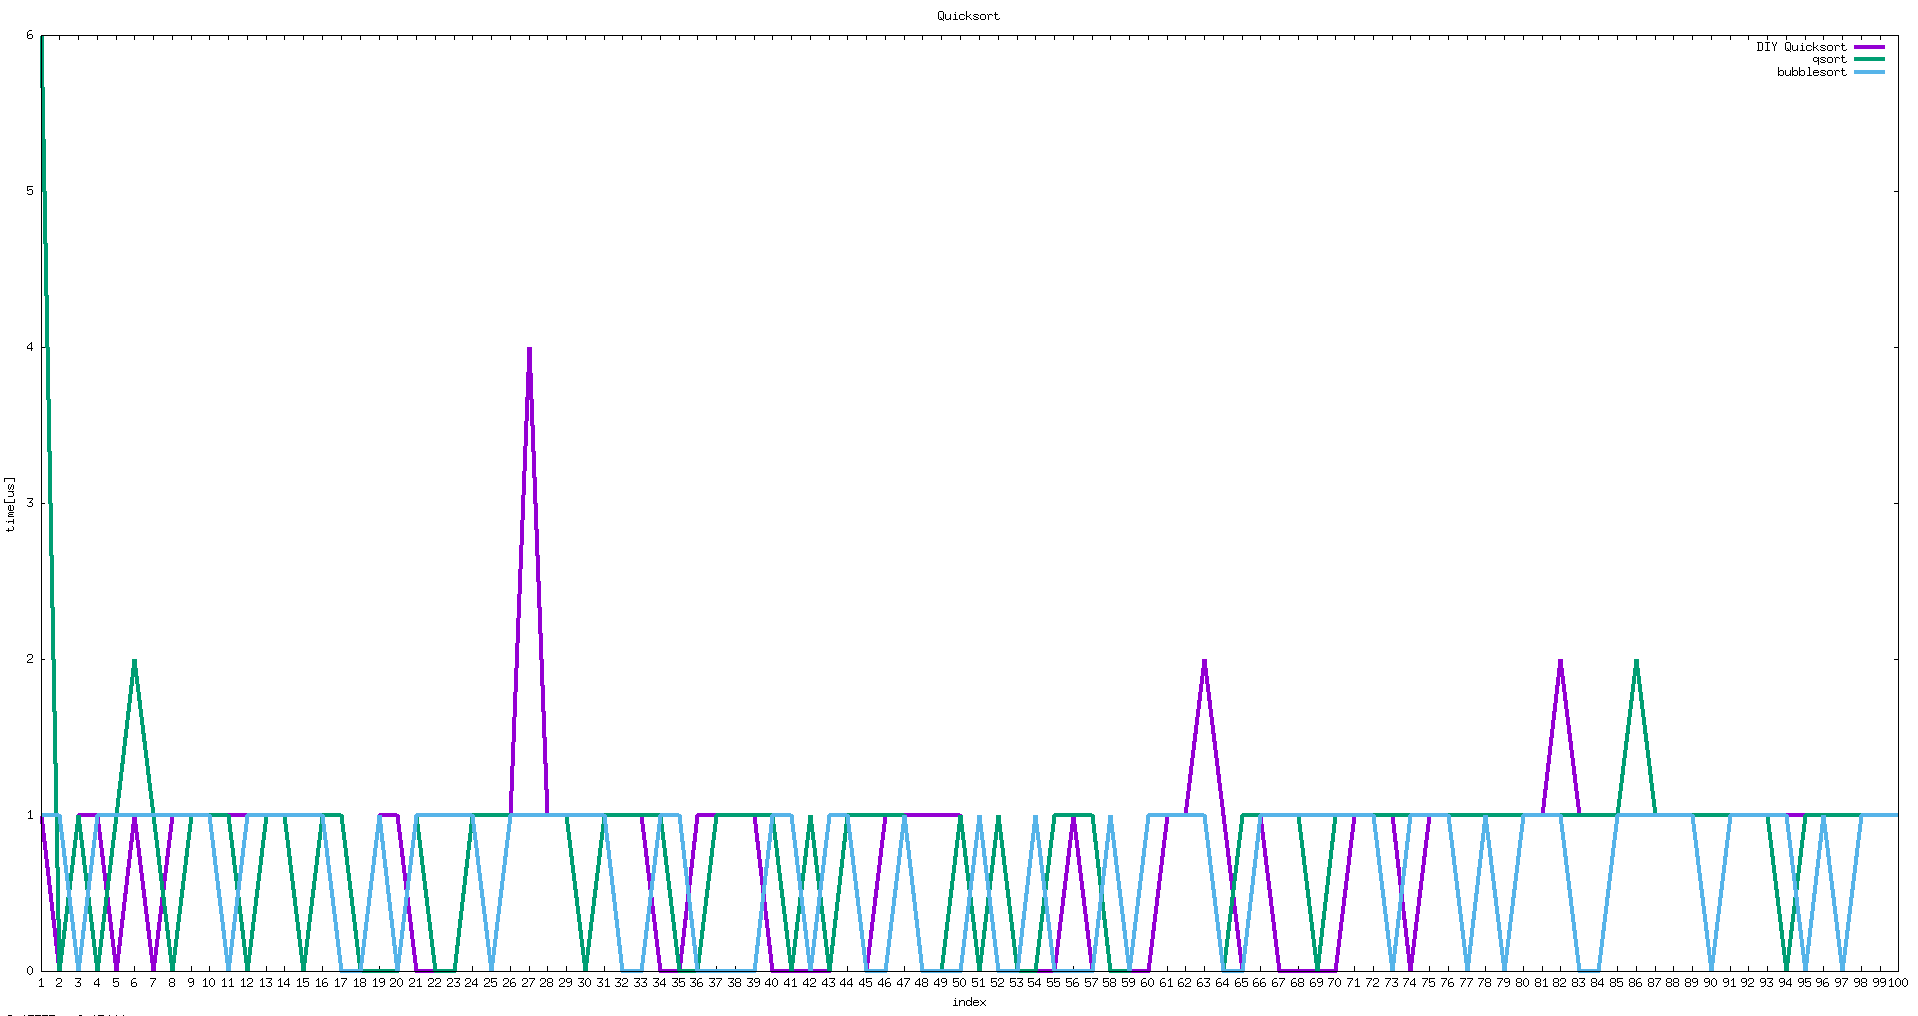
\includegraphics[width=\linewidth]{Sortieren-10.png}
        \caption{Sortieren-10}
        \label{caption:Sortieren-10}
    \end{figure}
    
\newpage
    \begin{figure}[!htb]
        \centering
        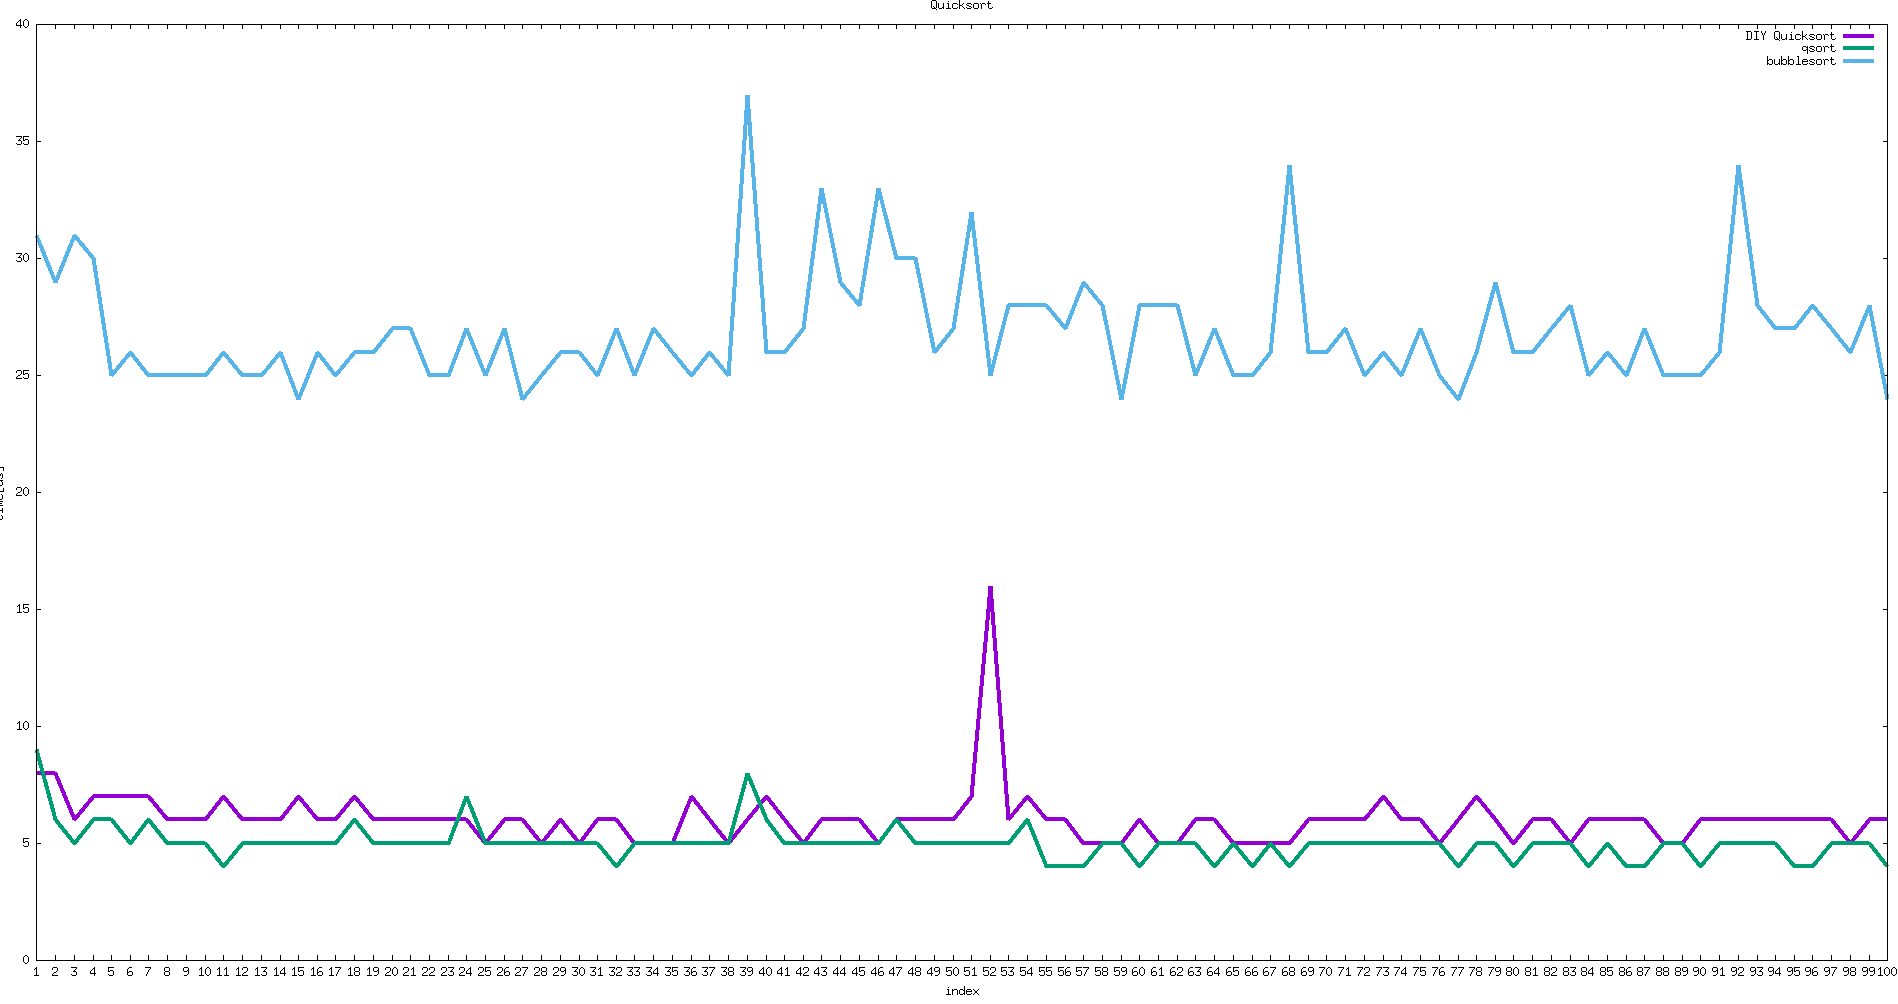
\includegraphics[width=\linewidth]{Sortieren-100.png}
        \caption{Sortieren-100}
        \label{caption:Sortieren-100}
    \end{figure}
    
    \begin{figure}[!htb]
        \centering
        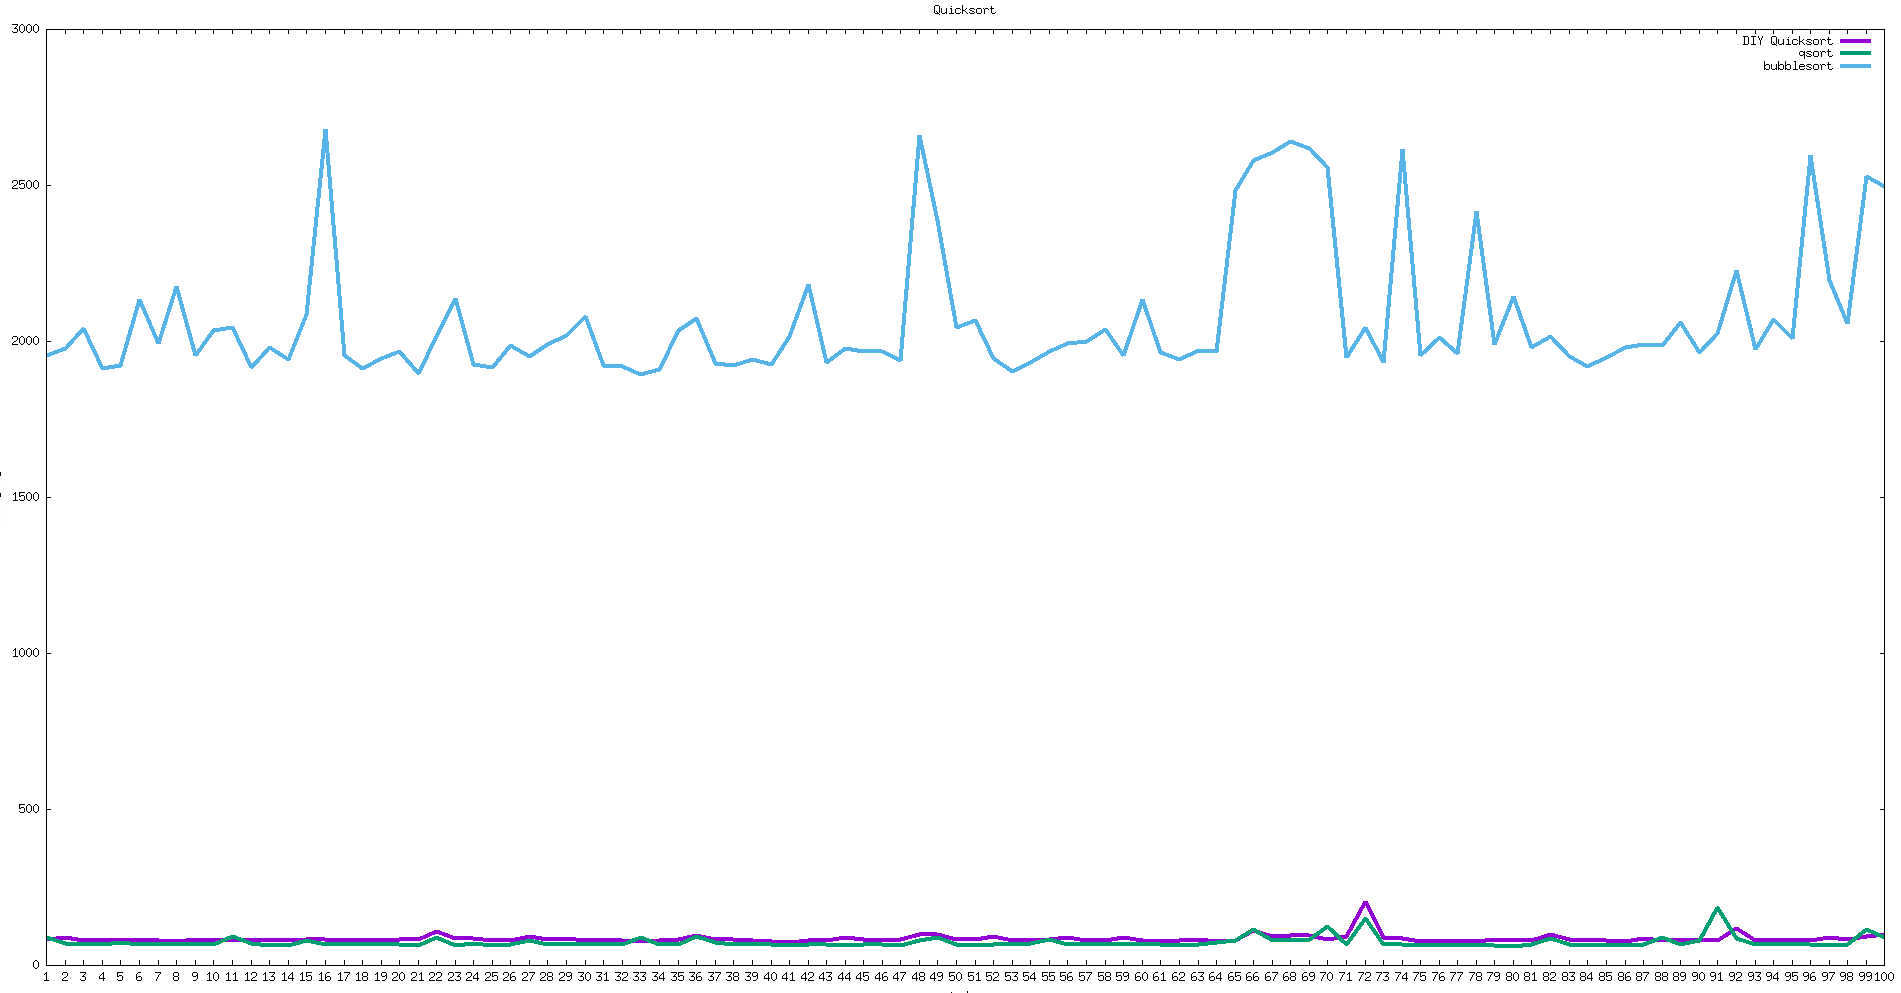
\includegraphics[width=\linewidth]{Sortieren-1000.png}
        \caption{Sortieren-1000}
        \label{caption:Sortieren-1000}
    \end{figure}
    
\newpage
    \begin{figure}[!htb]
        \centering
        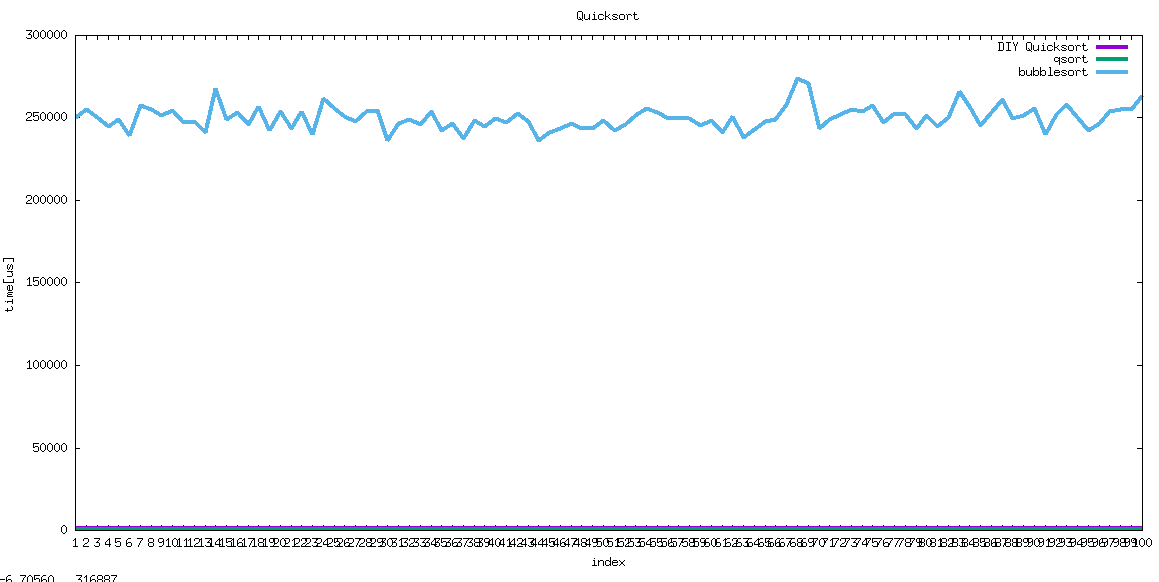
\includegraphics[width=\linewidth]{Sortieren-10000.png}
        \caption{Sortieren-10000}
        \label{caption:Sortieren-10000}
    \end{figure}
    
    \begin{figure}[!htb]
        \centering
        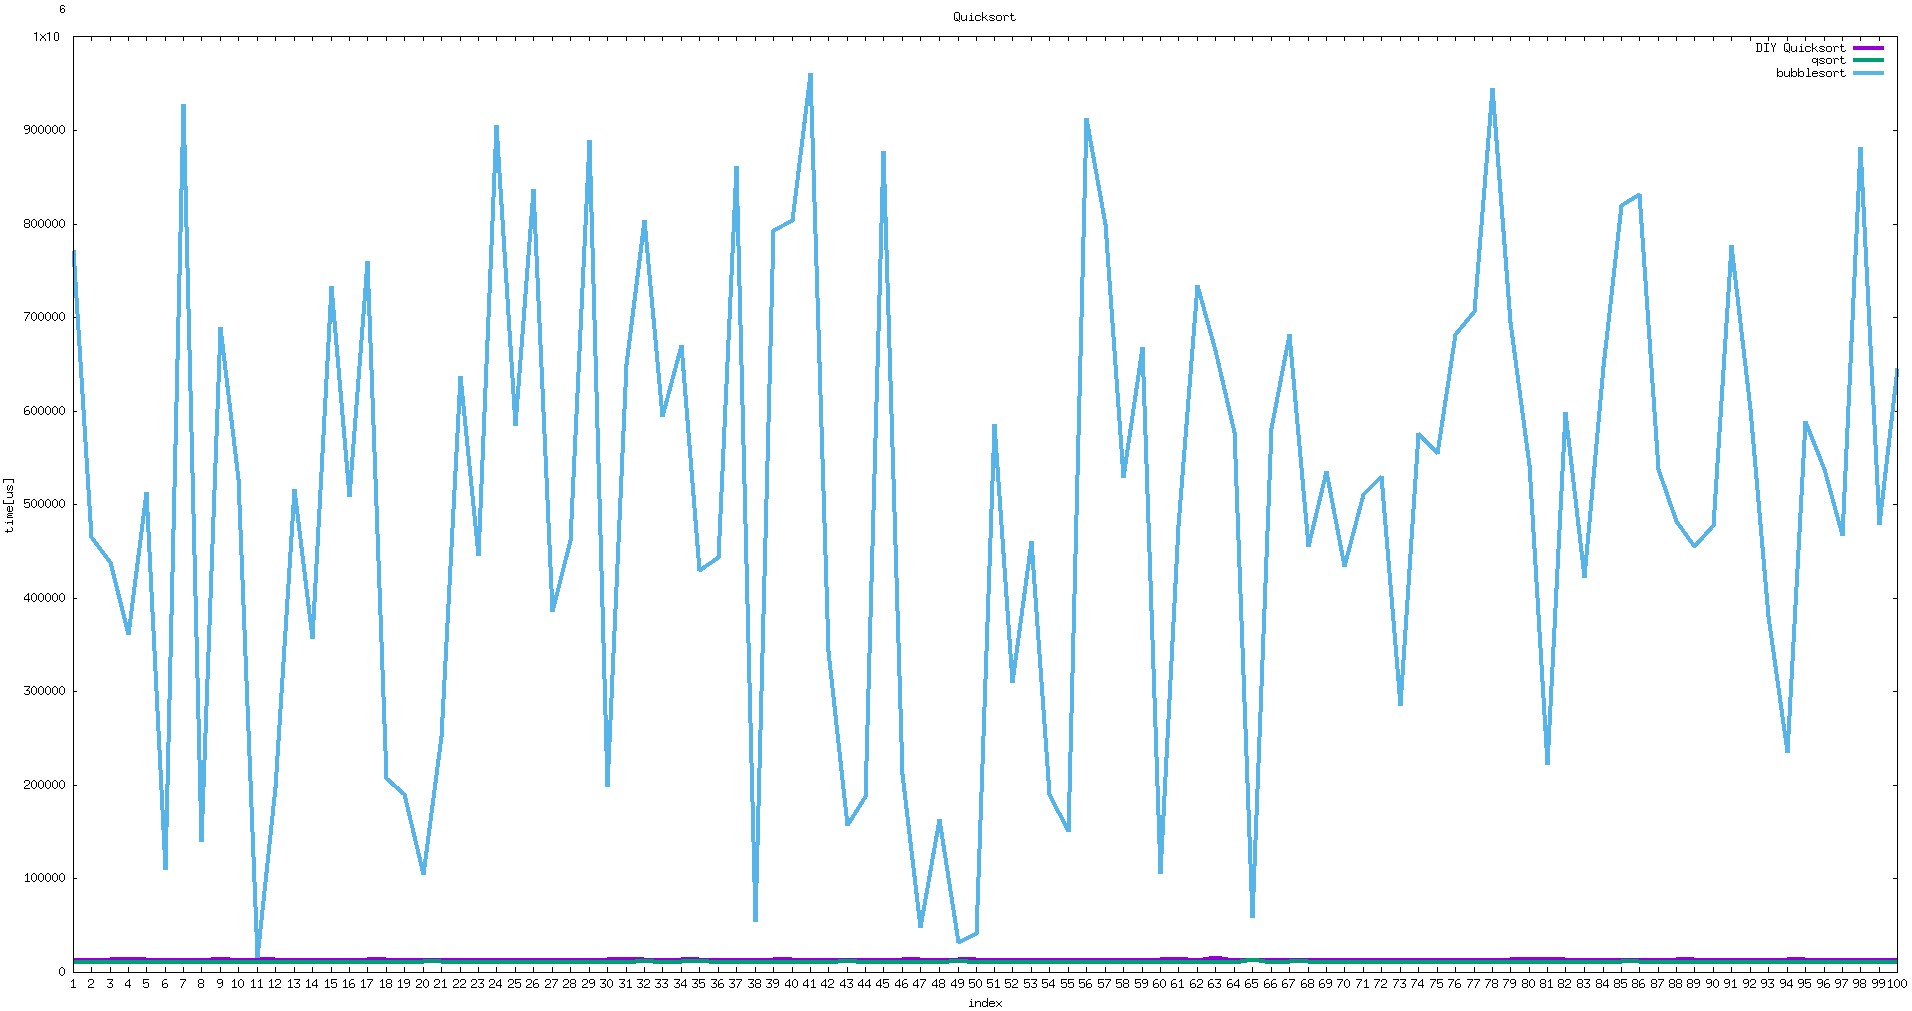
\includegraphics[width=\linewidth]{Sortieren-100000.png}
        \caption{Sortieren-100000}
        \label{caption:Sortieren-100000}
    \end{figure}
    
\newpage
    \noindent Man sieht, das BubleSort immer langsamer wird bei einer Array Größe von 1000 Zahlenwerten benötigt es schon ca. $2500\mu s = 0,0025s$\\
    Bei einer Anzahl von 10000 Werten sind es schon $250000\mu s = 0,25$. Das sind über 4 Minuten.\\
    Bei einer Array Größe von 100000 schwank BubleSort sehr stark von einmal gleich schnell wie QSort bis zu $900000\mu s = 0,9$.





\end{document}
